\documentclass[11pt]{article}
\usepackage{graphicx}
\usepackage[margin=3cm]{geometry}
\usepackage[usenames,dvipsnames]{color}
\usepackage{array}
\usepackage[colorlinks=true, urlcolor=MidnightBlue]{hyperref}
\usepackage{fancyhdr}

%%% Measurements %%%
\topmargin=-0.3in
\oddsidemargin=0in
\evensidemargin=0in
\textwidth=6.5in
\marginparwidth=0.5in
\headheight=0pt
\headsep=0pt
\textheight=9.0in

%%% Table formatting %%%
\definecolor{lightgray}{gray}{0.8}
\newcolumntype{L}{>{\raggedleft}p{0.14\textwidth}}
\newcolumntype{R}{p{0.8\textwidth}}
\newcommand\VRule{\color{lightgray}\vrule width 0.5pt}

\title{JAMIE A. MACDONALD}
\author{\href{mailto:jamie.alban@gmail.com}{jamie.alban@gmail.com}\\(613) 583-7654\\2251 Fife Cres.\\Ottawa, ON\\K1G 2Z3}
\date{}

\renewcommand{\headrulewidth}{0pt} % no rule for header

\lfoot{\href{https://twitter.com/JamieMacdo}{@JamieMacdo}}
\cfoot{\href{https://github.com/jameh}{github.com/jameh}}
\rfoot{\href{https://ca.linkedin.com/in/jamiemacdo/}{ca.linkedin.com/in/jamiemacdo/}}

\begin{document}
%%% Center Name and email %%%
\begin{minipage}{0.2\textwidth}
\hspace{0em}
\end{minipage}
%%% Name and email %%%
\begin{minipage}{0.55\textwidth}
\vspace{-3em}
\maketitle
\end{minipage}
%%% Picture %%%
\begin{minipage}{0.25\textwidth}
\flushright{
    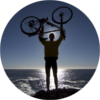
\includegraphics
    {jamie_alban_small.png}
}
\end{minipage}
\thispagestyle{fancy}
\vspace{-2.5em}
\section*{Objective}
I am looking for \textbf{fast-paced} summer employment in the field of \textbf{Software Development}. I have a strong \textbf{math and programming background} from my studies and hobbies, and I am excited by clean, simple, \textbf{innovative} solutions to human problems.
\section*{Education}
\begin{tabular}{L!{\VRule}R}
2010--2014&{\bf BSc Mathematics \& Engineering, Computing and Communication}\\
          &{Queen's University, Kingston Ontario}\\
\end{tabular}
\section*{Programming}
\textbf{Git}; \textbf{Python} web development in Django, Flask; OOP; scripting; Abstract Syntax Tree parsing; Closures; Decorators; list comprehensions; Matplotlib, Scipy, Numpy; Sphinx; \textbf{bash} automation; scripting; \textbf{C} Makefiles; compiler flags; memory management; \textbf{Java} Generics, Interfaces, Polymorphism, swing; \textbf{C++} OOP; \textbf{Javascript} Coffeescript; event handlers; \textbf{HTML, CSS} Liquid, Jinja templates; SCSS; Box model; \textbf{Octave, Matlab}; \textbf{LaTeX}

\section*{Projects}
\begin{tabular}{L!{\VRule}R}
2013--2014&{\bf Channel-Optimized Vector Quantization of Correlated Images for Transmission over a Wireless Channel (Fourth Year Project/Thesis)}\\
          &{Implement a Lossy Joint Source-Channel Code which exploits the Correlation in two random sources (images)}\\
          &{(Information Theory, C programming, Python matplotlib, LaTeX writeup)}\\
2010&{\bf Child Soldier Cycle}\\
    &{Biked 3000km from Ottawa to Newfoundland running an awareness campaign for child soldiering -- collected over 1500 red handprints as a petition to the media to provide better coverage of global Child Soldiering issues}
\end{tabular}


\section*{Activities}
\textbf{Open Source contributions}: Openbox (C), Nitrogen (C++ GTK)\\
\textbf{Clubs}: Queen's Hack Nights\\
\textbf{Recreation}: Rockclimbing, Biking\\
\textbf{Blog}: \href{http://jameh.github.io}{http://jameh.github.io} (Jekyll, SCSS, Liquid, Markdown)

\end{document}
